%-------------------------------------------------------------------------------
\section{Working Example}
%-------------------------------------------------------------------------------

\begin{figure}
  \centering
  \begin{subfigure}[b]{0.48\columnwidth}
    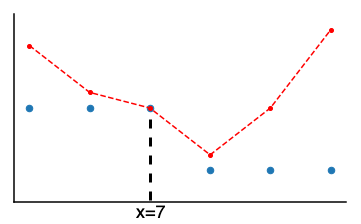
\includegraphics[width=\linewidth]{figs/sosp-working_ex3}
    \caption{\label{fig:working_ex1}Proximal cost function at $\bar{x} = 7$.}
  \end{subfigure}
  \hspace{0.1cm}
  \begin{subfigure}[b]{0.48\columnwidth}
    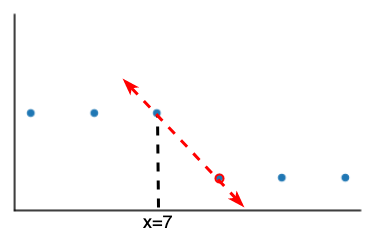
\includegraphics[width=\linewidth]{figs/sosp-working_ex2}
    \caption{\label{fig:working_ex2}Evaluated Proximal Gradient for $\bar{x} = 7$.}
  \end{subfigure}
  \vspace{-15pt}
  \caption{\label{fig:working_ex}Example of Proximal Gradient Evaluation.}
  \vspace{-15pt}
\end{figure}

To give a better intuition for how proximal gradients work in practice, we provide a working example. Consider the function $f(x) =   x \texttt{\&} 4$ shown in figure \ref{fig:ex_funcs}, and suppose we are evaluating it with $\bar{x} = 7$. This type of bitwise operation is common in programs that parse a file for input, since they frequently need to check if flag bits are set in a header or section header of the file. However, discrete functions like bitwise operations are nondifferentiable so we instead evaluate the proximal gradient.

To evaluate the proximal gradient on $f\left(x\right)$, the sampling region must first be defined. \tc{x \& 4} has a Lipschitz Constant of $K=4$ (any bitwise operation with a constant has a Lipschitz Constant with the value of the most significant bit in the constant), so assuming a proximal scaling factor of $\lambda = 1$, the sampling distance bound is $2K = 8$. Therefore, a total of 16 samples must be taken, for $x = [-1, 15]$, and the cost function of the proximal operator, $f(x) + ||x - \bar{x}||_2^2$ evaluated for each possible $x$. Figure \ref{fig:working_ex1} shows the value of the cost function near $x = 7$, there is a clear minimum at $x=8$, where $f\left(8\right) + ||8-7||_2^2 = 1$, so the proximal operator evaluates to $x=8$. The proximal gradient is then $prox_{\nabla f}\left(7\right) = \frac{f\left(7\right) - f\left(8\right)}{7 - 8} = -4$.


